% !TEX root = 0_main.tex
\chapter{Global Flow}\label{chap:global}
The global flow of \sys{} is shown in \fig{fig:globalflow}.
It consists of the following four steps:

\begin{figure*}
\centering
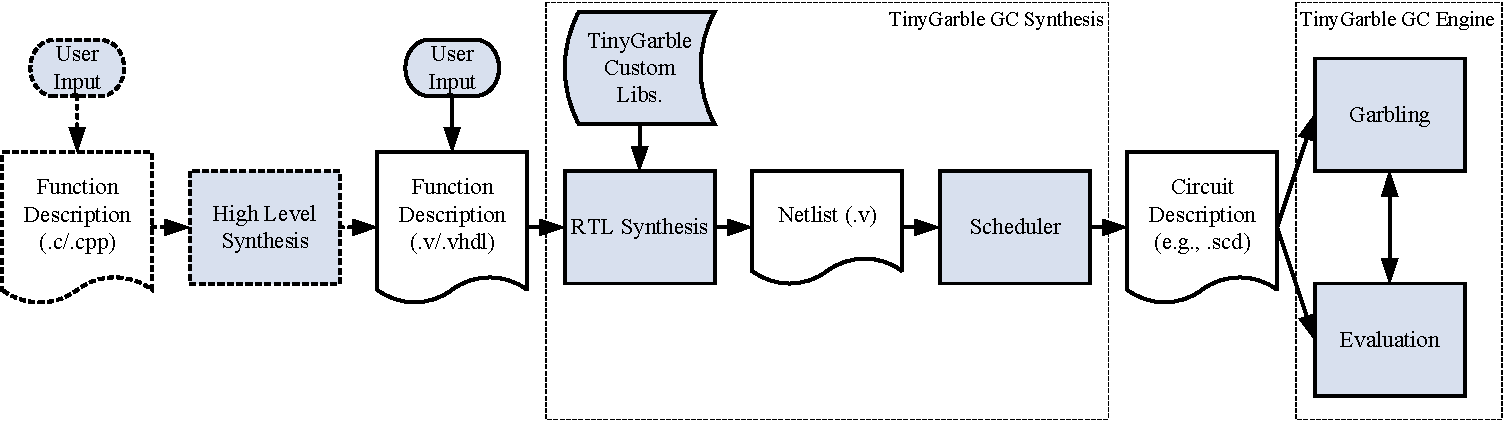
\includegraphics[width=0.95\textwidth]{flow_chart-crop.pdf}
\caption{Global flow of \sys{} for both combinational and sequential synthesis.
  The inputs can be either a C/C++ program (translatable to HDL via a standard HLS tool) or a direct HDL description.
  \sys{} is able to provide circuit description for any given GC framework.}
\label{fig:globalflow}
\end{figure*}

\begin{enumerate}
\item
  The input to the \sys{} framework is a file that describes a sequential or combinational function written in an HDL like Verilog or VHDL.
  The function can also be written in a high level language like C/C++ and automatically translated to HDL using an HLS tool.
  In the sequential circuit, the degree of folding is specified by the user.

\item
  A standard HDL synthesis tool compiles the HDL to generate a netlist file.
  The synthesis tool optimizes the netlist based on the user defined objectives/constraints and a customized library.

\item
  The netlist is parsed and topologically sorted.
  If the circuit is sequential, only its combinational part is sorted.
  Then, the sorted netlist is saved in a format compatible with any given GC framework e.g., Simple Circuit Description (SCD) compatible with JustGarble~\cite{bellare2013efficient}.

\item
  The circuit description is provided to both the garbler and evaluator to securely evaluate the function by the GC framework.
\end{enumerate}

\begin{figure*}
\centering
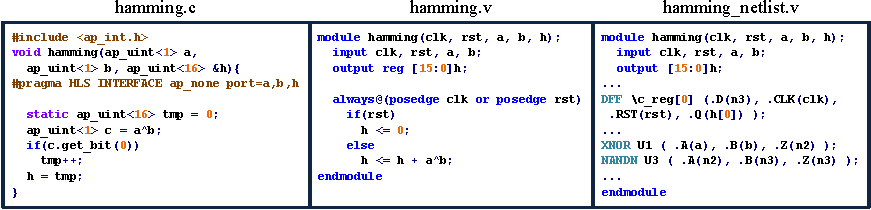
\includegraphics[width=\textwidth]{HLS_HDL_netlist-crop.pdf}
\caption{Sample files at the different steps of \sys{}'s flow for Hamming distance function.}
\label{fig:globalflow_sample}
\end{figure*}

\fig{fig:globalflow_sample} shows examples of files at different steps of \sys{}'s flow for the Hamming distance function.
The \textsl{hamming.c} file contains the description of the function in the C language.
The user inputs this function to a HLS tool to generate the corresponding description in Verilog.
The resulting Verilog file is functionally similar to the \textsl{hamming.v} file shown in the figure, but it may look more complicated and be less efficient as it is generated by an automated tool.
A user can also write the description directly in Verilog to have more control on the circuit and therefore a more efficient netlist.
The \textsl{hamming.v} file is provided to an HDL synthesis tool along with the \sys{} custom libraries to generate netlist \textsl{hamming\_netlist.v}.
The netlist describes the same function as \textsl{hamming.c} and \textsl{hamming.v} but uses the logic cells provided in the technology library.
The technology library contains 2-input-1-output logic cells to be compatible with front-end garbling tools~\cite{malkhi2004fairplay, bellare2013efficient}.
